\documentclass{article}
\usepackage{graphicx} 

\title{Final Report}
\author{Aaenoor Saqib}
\date{June 2023}

\begin{document}

\maketitle

\section{Introduction}
This is my final report on the Computer Lab Module. It contains an overview of all the topics covered and all the skills I have learned in this module.

\section{Week 1: Introduction}
Week one was an intro week where we talked about what we would learn in this module. We discussed online portfolios and how they are important to us, especially for software engineering students.

\section{Week 2: Touch Typing}
This week, we talked about touch typing. Specifically, we discussed its origins, types of typing techniques, and the importance of touch typing for our future. We were also given a task to record our progress over the course of the semester. The table below shows my progression.

% Insert Week 2 image here
\begin{figure}[ht]
  \centering
  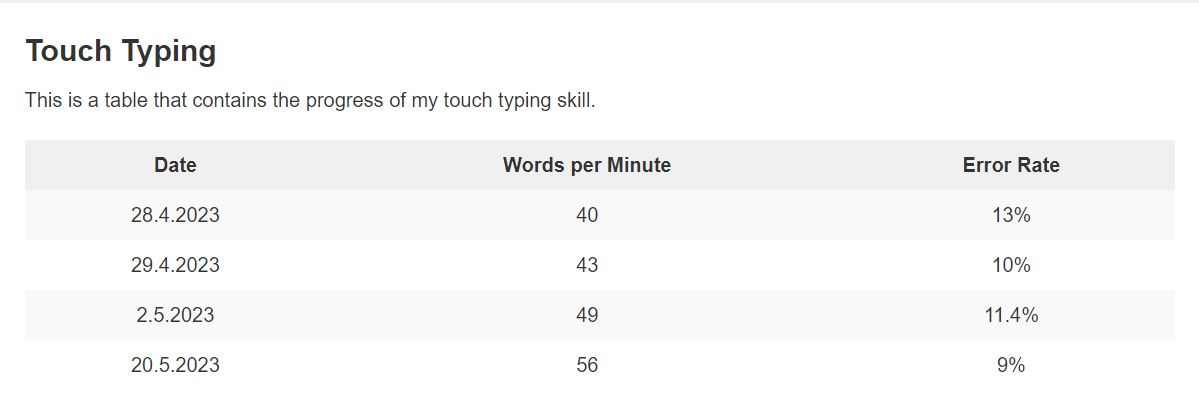
\includegraphics[width=0.5\textwidth]{touch typing table ss}
  \caption{touch typing table progress}
  \label{fig:week2_image}
\end{figure}

\section{Week 3: LaTeX}
In week 3, we learned about LaTeX. We explored what LaTeX is, its applications across different fields, and how we can use it. We created our CVs using templates on Overleaf, which helped us become familiar with LaTeX and ultimately facilitated the writing of this report.

% Insert Week 3 image here
\begin{figure}[ht]
  \centering
  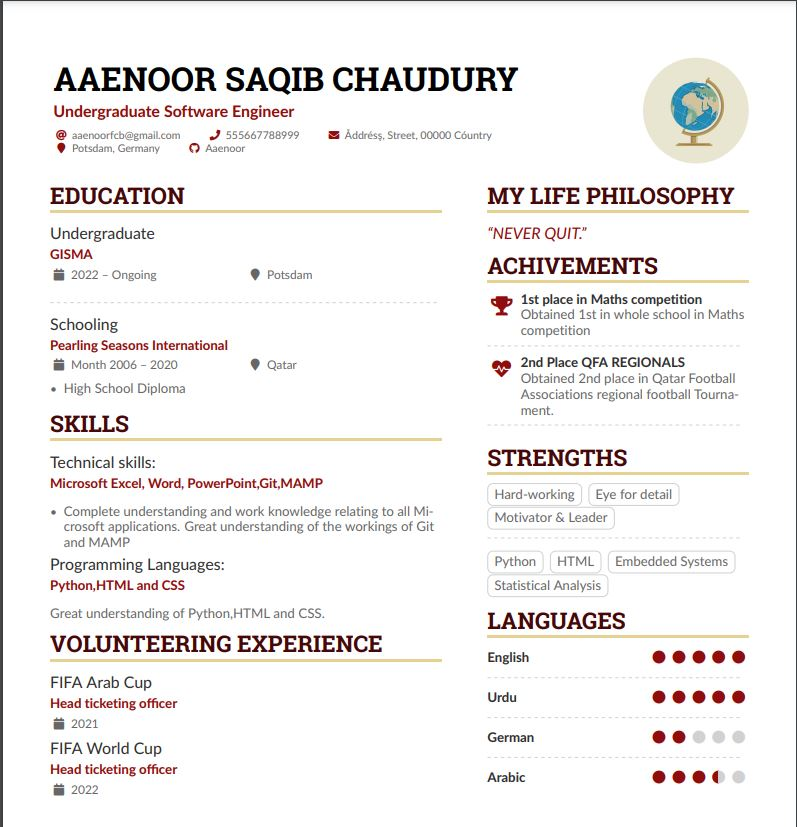
\includegraphics[width=0.5\textwidth]{CVss}
  \caption{CV i made using Overleaf template.}
  \label{fig:week3_image}
\end{figure}

\section{Week 4: Linux}
Week 4 was dedicated to learning about Linux. We delved into various aspects of Linux, including its command-line interface, file system, and basic commands. We gained practical experience with Linux by performing tasks and exercises related to system administration.



\section{Week 5: HTML and CSS}
In week 5, we focused on HTML and CSS. This was one of the most beneficial weeks for me, as we learned how to write HTML and CSS code. We were assigned to create a website for our portfolios using HTML and style it using CSS. Additionally, we learned about merging and other related concepts in HTML and CSS.

\section{Week 5: HTML and CSS}
In week 5, we focused on HTML and CSS. This was one of the most beneficial weeks for me, as we learned how to write HTML and CSS code. We were assigned to create a website for our portfolios using HTML and style it using CSS. Additionally, we learned about merging and other related concepts in HTML and CSS.

\begin{figure}[ht]
  \centering
  \begin{minipage}{0.45\textwidth}
    \centering
    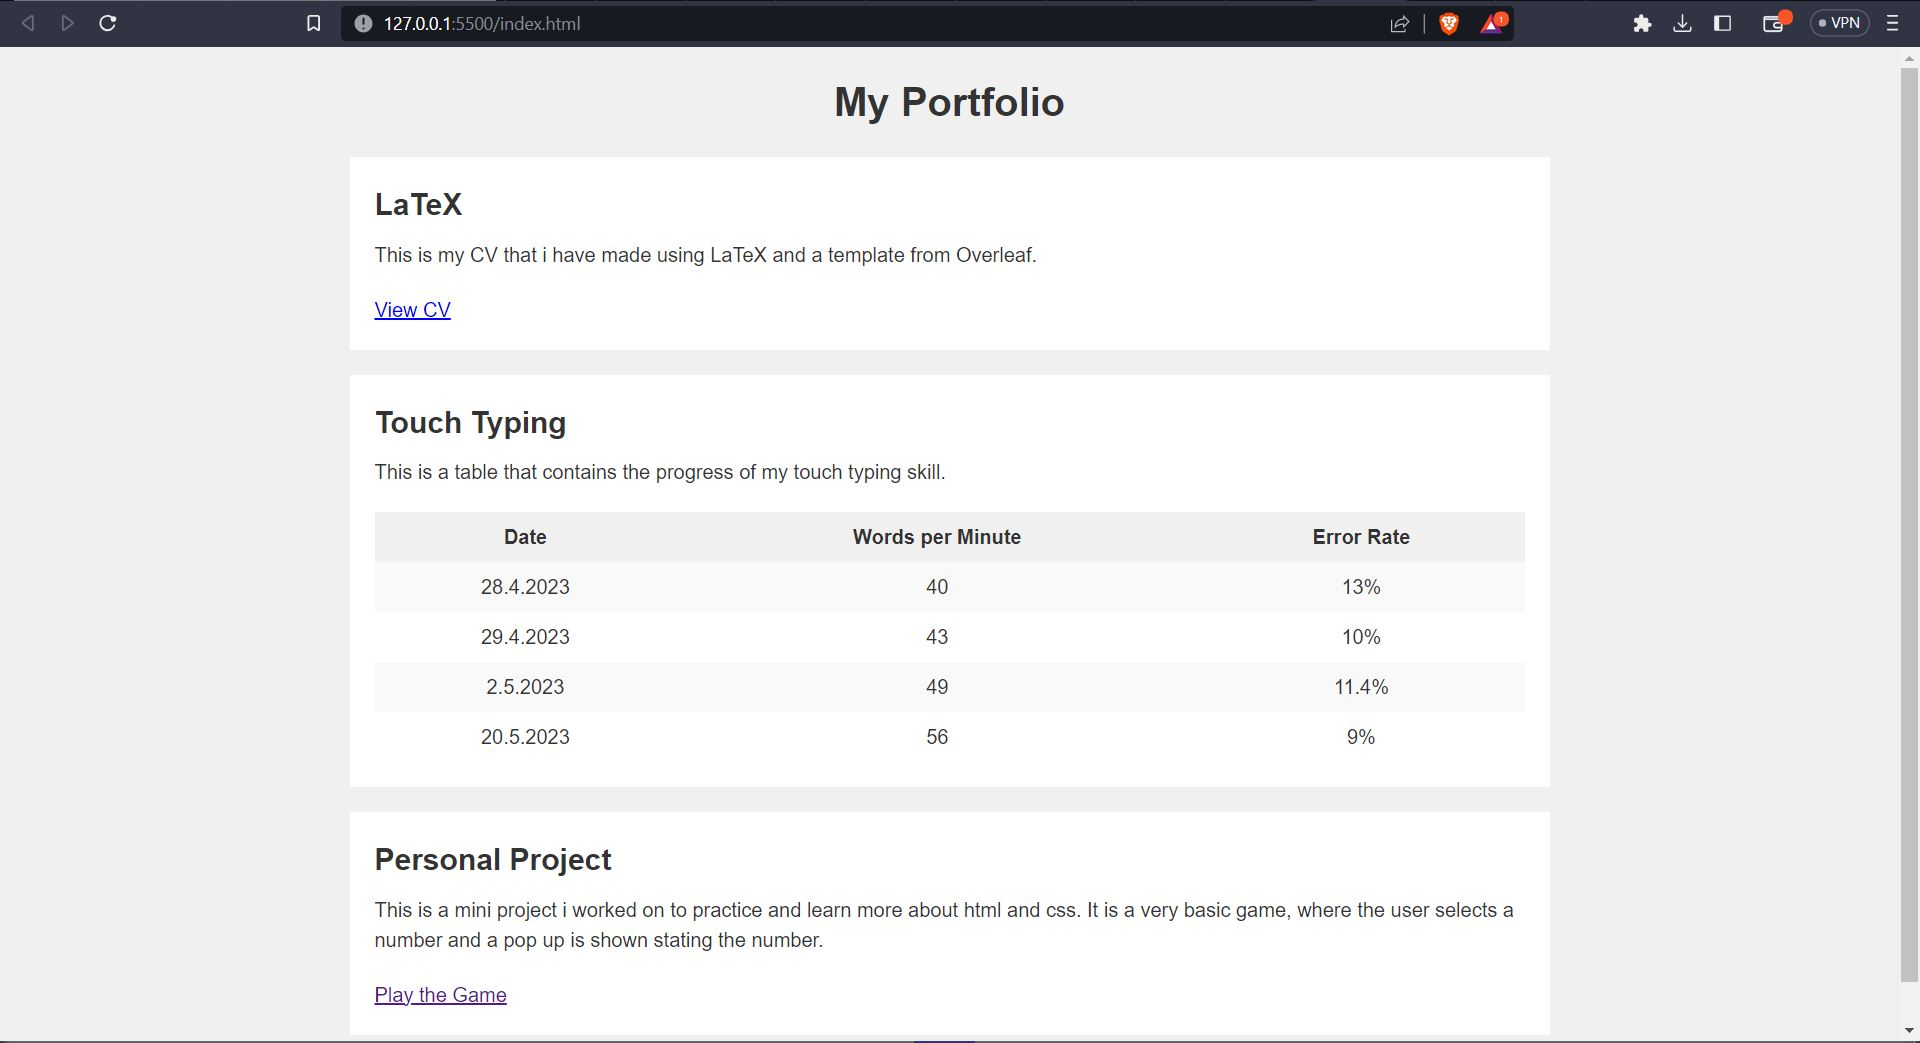
\includegraphics[width=\textwidth]{website ss}
    \caption{Caption describing the image for Week 5.}
    \label{fig:week5_image}
  \end{minipage}\hfill
  \begin{minipage}{0.45\textwidth}
    \centering
    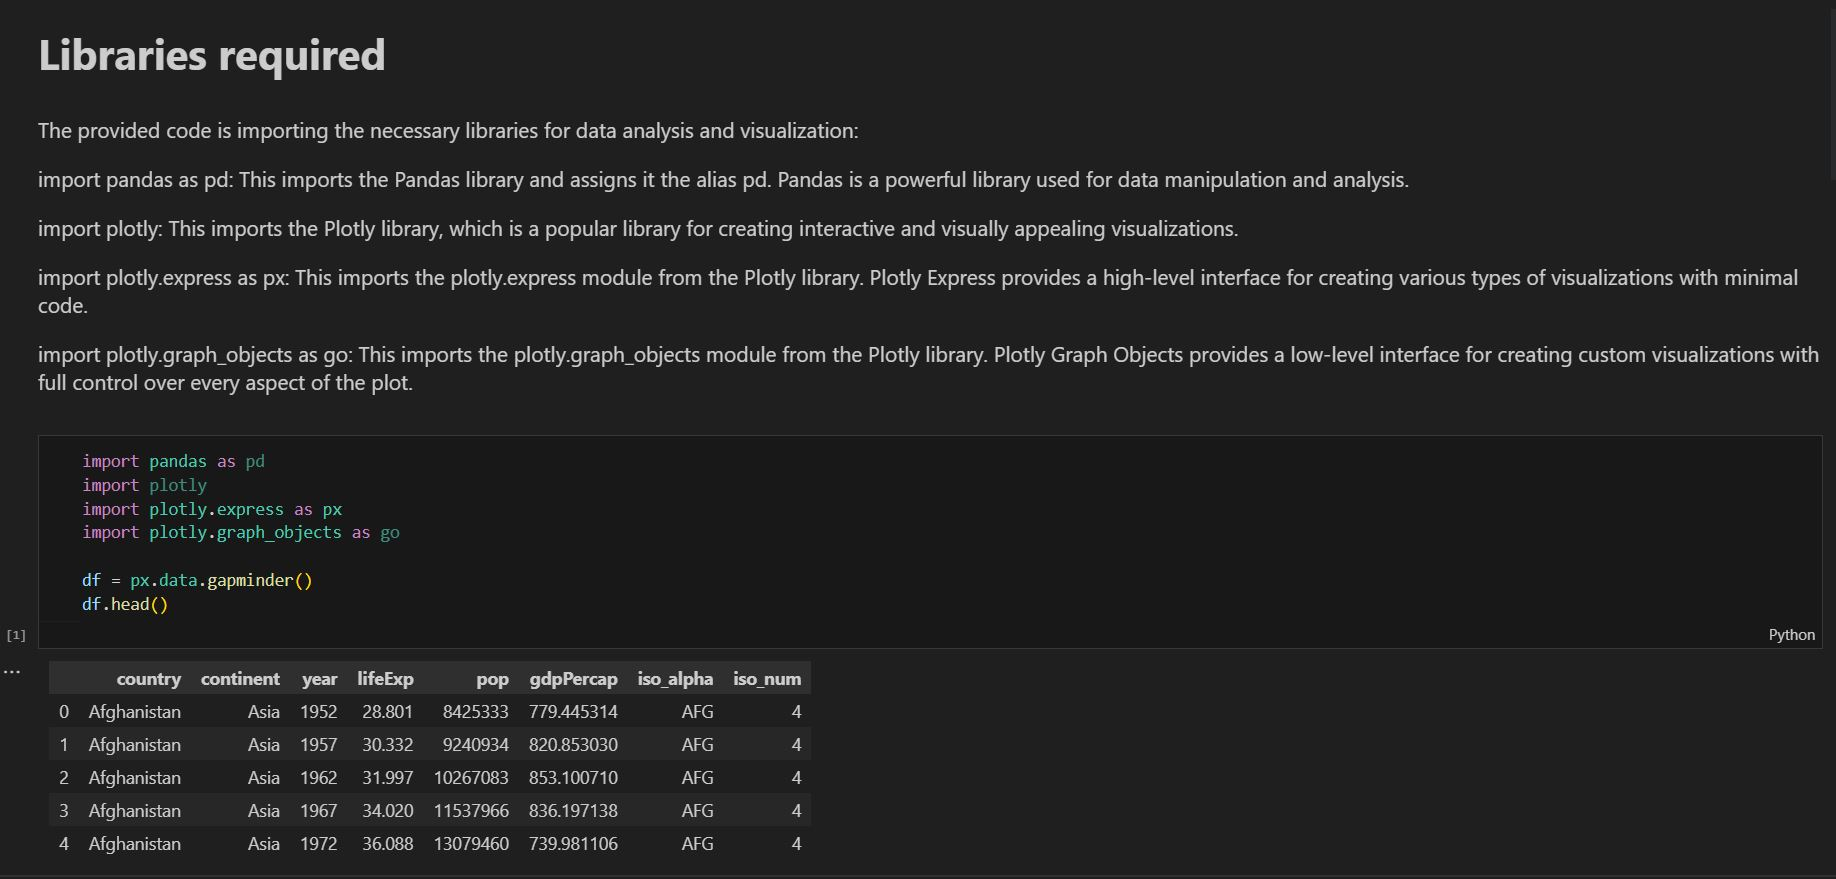
\includegraphics[width=\textwidth]{JH pt1}
    \caption{My website made using HTML and CSS}
    \label{fig:week5_mini_project_image}
  \end{minipage}
\end{figure}
  

\section{Week 6: Jupyter}
During week 6, we explored Jupyter and its applications in data analytics. We learned how to create and work with Jupyter notebooks, allowing us to evaluate and analyze data. A project was assigned to us that involved working with Pandas and Plotly to analyze data and create visualizations.

\begin{figure}[ht]
  \centering
  \begin{minipage}{0.45\textwidth}
    \centering
    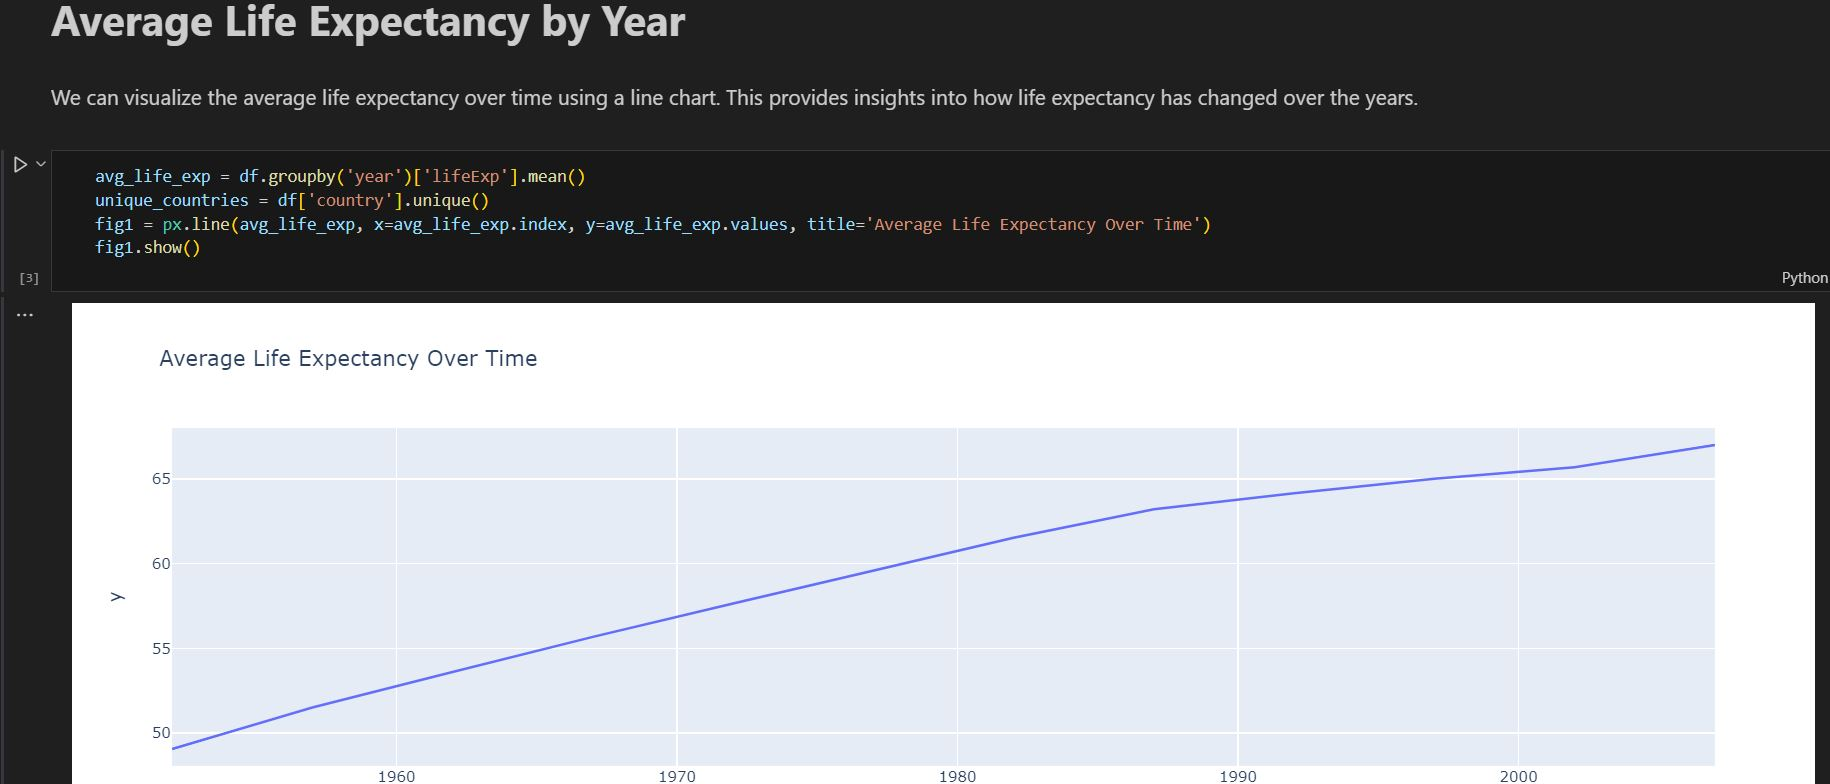
\includegraphics[width=\textwidth]{JH Pt3}
    \caption{Caption describing the image for Week 6.}
    \label{fig:week6_image}
  \end{minipage}
\end{figure}

\section{Week 7: Git}
Week 7 focused on Git, which was an interesting and valuable week for me. We covered various aspects of Git, including creating repositories, the staging process, and other useful Git commands. We gained a comprehensive understanding of how Git can be beneficial for software developers.



\section{Week 8: GitHub}
During week 8, we learned about GitHub and its applications. We were instructed to create a GitHub account and upload all our module tasks to create a portfolio. GitHub provides an excellent platform for showcasing our work and collaborating with other developers.

Here is a link to my GitHub account: \url{https://github.com/Aaenoor/Portfolio}

\section{Conclusion}
Overall, the Computer Lab Module was well-structured and effectively taught by the professor. It provided valuable skills and knowledge for individuals at all levels of coding and those interested in software engineering and other branches of IT. The module did an amazing job of teaching the fundamental skills and knowledge required to succeed in this field.

In conclusion, I would like to express my gratitude for the opportunity to participate in this module and extend my appreciation to the professor for their guidance and expertise.

\end{document}
